%% latex_185_moulds_g.tex
%%
%% The following file is a skeleton file that demonstrates how to implement the IEEEtran.cls class 
%% file in LaTeX. This file is intended for the CMPE185 Technical Writing for Engineers Course in 
%% which the students must write a tutorial aimed towards novice LaTeX users in the LaTex environment.
%%
%% This file is heavily adapted from Michael Shell's bare_adv.tex file made available at 
%% http://www.ieee.org/conferences_events/conferences/publishing/templates.html
%%
%% You will need to rename this file with your information in the following format:
%% latex_185_last name_ first initial.tex
%% ---------------------------------------------------------------------------------------------------

% \documentclass{} precedes the preamble and is typically the first command in any .tex document. Every .tex document should include this command as it defines what kind of document you intend on creating. Modifiers in square brackets [] can be added in between the text ''documentclass'' and the curly brackets {} to modify font size, templates, etc. 

\documentclass[12pt,journal,compsoc]{IEEEtran}

%-----PACKAGES-------------------------------------------------------------------------------------

% Packages include extra commands that allow for additional formatting, ranging from Graphics, Math, to Alignment. The command to include packages will always look similar to \usepackage{} where the package name is within the curly brackets {}. Packages are defined in the preamble, i.e., between the \documentclass{} and \begin{document} commands.

% The following link takes you to a list of additional packages that may not be listed here. http://en.wikibooks.org/wiki/LaTeX/Package_Reference

% TO INCLUDE PACKAGES: 
% - Open the file ''latex_sample_packages.tex'' from the .zip folder.
% - From this file, COPY the code for the package you want to include and PASTE into your own .tex file.
% - Uncomment the package you want to include and load, i.e., remove the ''%'' in front of the \usepackage{package_name}.
 

% Copy package text here:

\usepackage{graphicx}
% This is an example of how a \usepackage{} command should be included. You will need to include more packages to complete this assignment.

\usepackage{mathtools}


%----- The DOCUMENT Environment-------------------------------------------------------------------

% The \begin{document} and \end{document} commands establish the environment for the text of the document. The \begin{} and \end{} commands are used repeatedly in LaTeX to show where an environment begins and ends. The \end{document} command will be the last line of this .tex file.

\begin{document}

% The following commands are self explanatory. Insert your title, author and date into each command's curly bracket. You can include the abstract, paper header and paper footer information in this section then conclude the section with the command \maketitle (shown as the last line at the end of this section).

\title{Latex Tutorial}
\author{James~Pretti}
% The double backslash \\ is used here to enter a ''Carriage Return'', or a line break. Note that the tilde ~ in between my name used as a ''Nonbreaking Space''. LaTeX will not break a structure at a ~ so this keeps an author's name from being broken across two lines. Also note that I included my name as an example so make sure to only insert your name in this command.

\date{\today}		% leaving the brackets empty omits the date
% To input the current date, you can type: \date{\today}

% The paper headers
\markboth{\LaTeX\ IEEE Template Tutorial}%
{Moulds \MakeLowercase{\textit{et al.}}: CMPE185}
% The only time the second header will appear is for the odd numbered pages
% after the title page when using the twoside option.
% 
% *** Note that you probably will NOT want to include the author's ***
% *** name in the headers of peer review papers.                   ***
% You can use \ifCLASSOPTIONpeerreview for conditional compilation here if
% you desire.

% The publisher's ID mark at the bottom of the page is less important with
% Computer Society journal papers as those publications place the marks
% outside of the main text columns and, therefore, unlike regular IEEE
% journals, the available text space is not reduced by their presence.
% If you want to put a publisher's ID mark on the page you can do it like
% this:
%\IEEEpubid{0000--0000/00\$00.00~\copyright~2007 IEEE}
% or like this to get the Computer Society new two part style.
%\IEEEpubid{\makebox[\columnwidth]{\hfill 0000--0000/00/\$00.00~\copyright~2007 IEEE}%
%\hspace{\columnsep}\makebox[\columnwidth]{Published by the IEEE Computer Society\hfill}}
% Remember, if you use this you must call \IEEEpubidadjcol in the second
% column for its text to clear the IEEEpubid mark (Computer Society jorunal
% papers don't need this extra clearance.)


% use for special paper notices
%\IEEEspecialpapernotice{(Invited Paper)}

% for Computer Society papers, we must declare the abstract and index terms
% PRIOR to the title within the \IEEEcompsoctitleabstractindextext IEEEtran
% command as these need to go into the title area created by \maketitle.
\IEEEcompsoctitleabstractindextext{%
\begin{abstract}
%\boldmath
The following document was written with the intent of educating novice engineering students on the creation of documents using LaTeX.
\end{abstract}
% IEEEtran.cls defaults to using nonbold math in the Abstract.
% This preserves the distinction between vectors and scalars. However,
% if the journal you are submitting to favors bold math in the abstract,
% then you can use LaTeX's standard command \boldmath at the very start
% of the abstract to achieve this. Many IEEE journals frown on math
% in the abstract anyway. In particular, the Computer Society does
% not want either math or citations to appear in the abstract.

% Note that keywords are not normally used for peerreview papers.
\begin{IEEEkeywords}
CMPE185, \LaTeX\ Tutorial, IEEEtran, journal, \LaTeX, paper, template.
\end{IEEEkeywords}}

\maketitle

%----- The SECTION Environment -------------------------------------------------------------------

% To create a section, simply type the command \section{} with the name of your section name inserted into the curly brackets {}. The section's body text follows underneath the \section{} command. 

\section{Introduction}
% Computer Society journal papers do something a tad strange with the very
% first section heading (almost always called "Introduction"). They place it
% ABOVE the main text! IEEEtran.cls currently does not do this for you.
% However, You can achieve this effect by making LaTeX jump through some
% hoops via something like:
%
%\ifCLASSOPTIONcompsoc
%  \noindent\raisebox{2\baselineskip}[0pt][0pt]%
%  {\parbox{\columnwidth}{\section{Introduction}\label{sec:introduction}%
%  \global\everypar=\everypar}}%
%  \vspace{-1\baselineskip}\vspace{-\parskip}\par
%\else
%  \section{Introduction}\label{sec:introduction}\par
%\fi
%
% Admittedly, this is a hack and may well be fragile, but seems to do the
% trick for me. Note the need to keep any \label that may be used right
% after \section in the above as the hack puts \section within a raised box.



% The very first letter is a 2 line initial drop letter followed
% by the rest of the first word in caps (small caps for compsoc).
% 
% form to use if the first word consists of a single letter:
% \IEEEPARstart{A}{demo} file is ....
% 
% form to use if you need the single drop letter followed by
% normal text (unknown if ever used by IEEE):
% \IEEEPARstart{A}{}demo file is ....
% 
% Some journals put the first two words in caps:
% \IEEEPARstart{T}{his demo} file is ....
% 
% Here we have the typical use of a "T" for an initial drop letter
% and "HIS" in caps to complete the first word.

\IEEEPARstart{F}{irst} created in the early 1980's by Leslie Lamport, LaTeX was developed to aid in the production of general-purpose books and articles within TeX. Today, LaTeX is used by many people in the scientific community to publish scientific documents. One of the biggest benefits of using LaTeX is its ability to allow authors to include complicated mathematical equations, tables, figures, and non-Latin scripts in their writings. In addition to allowing the use of complicated symbols in its text, LaTeX also does something different than most text editors. LaTeX separates the formatting of a document from its content, allowing users to focus on both parts independently. This document will cover many of the important features and will act as a starting point for novice engineering students to create their first document in LaTeX. \cite{Wikipedia:Overview}
 

% Creating a subsection is similar to creating a section and is used with the command \subsection{}.

%\subsection{Subsection Heading Here}
%Subsection text here.

% needed in second column of first page if using \IEEEpubid
%\IEEEpubidadjcol

% Creating a subsubsection:

%\subsubsection{Subsubsection Heading Here}
%Subsubsection text here.


%----- Additional Features -----------------------------------------------------------------------

\section{Creating your first .tex file}

\subsection{Setup}
\subsubsection{Overleaf - Online LaTeX editor}
\IEEEPARstart{F}{or} this tutorial, I will be using an online LaTeX editor called Overleaf. Overleaf is a free editor that removes the need for separate LaTeX clients and LaTeX compilers. You can access Overleaf by signing up for a free account at \url{https://www.overleaf.com}

\subsubsection{File Structure}
The first command one should add to their .tex document is: \begin{verbatim} \documentclass[]{} \end{verbatim} This command defines the type of document to be created. Between the [ and ] characters, users can add document class options such as font size, paper size, page layout, etc. Between the \{ and \} characters, users can add their document class. \cite{Overleaf:Tutorial} Document classes instruct LaTeX to set the typeset of the document in a certain way to match specific classes like, article, IEEEtran, proc, etc. For this document, the package, IEEEtran, is being used. A full list of document class options and document classes can be found at: \url{https://en.wikibooks.org/wiki/LaTeX/Docu-
ment\_Structure}.\par

The second set of instructions a user should add are: 
\begin{verbatim}\begin{document}
...
\end{document} \end{verbatim} 
These instructions identify the start and end of your document. All of the content you create will go between these two instructions. \cite{Overleaf:Tutorial}

\subsubsection{Packages}
LaTeX's abilities only go so far. There are some instances where you may want to include things that basic LaTex is incapable of providing. To solve this, you can include additional enhancements called packages. The addition of various packages will allow users to accomplish things like adding graphics, colored text, or source code into their document. \cite{LaTeX2e:reference}
\\
\\
\par
To add packages to your document, use the command:
\begin{verbatim}\userpackage{package}\end{verbatim}
By replacing "package", in the command above, with the name of an actual package, your document will be able to use the additional functionality of that package. \cite{Overleaf:Tutorial}

\subsubsection{Adding Your Title}
The next step in your document creation is setting up your title information. To setup your title, enter the following commands:
\begin{verbatim}
\title{Your Title}
\author{Your~Name}
\date{}
\end{verbatim} 
Be sure to replace "Your Title" with an appropriate title for your document. When replacing "Your\~{}Name" with your actual name, you may want to include the \~{} symbol. This symbol makes LaTeX keep the word before and after it on the same line. Lastly you may enter any date you want in the date command; however, you may wish to have it automatically put in whatever today's date is. To do this use the command \cite{Overleaf:Tutorial}:
\begin{verbatim}
\date{\today}
\end{verbatim}
\par
Once you have successfully input your title, author, and date, it is time to give LaTeX the command to actually create your title heading. LaTeX will automatically format your title heading based on your current styling. To create your title heading, use the following command \cite{Overleaf:Tutorial}:
\begin{verbatim}
\maketitle
\end{verbatim}
*Warning* - You will get an error if you attempt to make title without including all the required title information, such as author. If you get this error, go back to your title heading and make sure you included all the necessary information. 

\subsubsection{Reserved Characters}
There are specific characters in LaTeX that command LaTeX to do certain things. These characters include the following:
\begin{verbatim}
\, ~, \\, %, #, $, ^, _, { and }
\end{verbatim}
For example, just typing \textbackslash{}, will make the editor think you are writing a command. Typing \~{} will make the editor think you are forcing two words onto the same line. Typing \textbackslash{}\textbackslash{} will make the editor think you are trying to create a new line. Typing a \% symbol will make the editor think you are trying to type a non-visible comment. If you wish to use these reserved characters in your text you will need to add a bit of extra code to have LaTeX interpret them as text rather than commands. The following reserved characters can be typed as text by simply adding a \textbackslash{} in front of them \cite{Overleaf:Tutorial}:
\begin{verbatim}
% , # , $ , _ , { and }
\end{verbatim}
To type the \textbackslash{} character as text, enter the following:
\begin{verbatim}
\textbackslash{}
\end{verbatim}
To type the text versions of \~{} and \^{}, enter the following:
\begin{verbatim}
\~{} and \^{}
\end{verbatim}
Finally, to type the text version of \textbackslash{}\textbackslash{}, type the following:
\begin{verbatim}
\textbackslash{}\textbackslash{}
\end{verbatim}

\subsubsection{Environments}
There will be times when you want to alter the appearance of a portion of text without editing the appearance of everything else. LaTeX makes this possible with the inclusion of environments. Environments allow users to format individual blocks of text. By using the following commands, you can setup your own environment block \cite{Overleaf:Tutorial}:
\begin{verbatim}
\begin{environment name}
...text...
\end{environment name}
\end{verbatim}
By replacing "environment name" in the code above with an actual environment name, you can assign the text written between \textbackslash{}begin and \textbackslash{}end{} to its own formatted environment. \cite{LaTeX2e:reference}
\par
You may wish to define your own environment. In this case, you would want to use the following command:
\begin{verbatim}
\newenvironment{environment name}
\end{verbatim}
On the next line you could then start to define your new environement. For example, let's create an environment called "myenvironment" and make its text centered and boxed. To do this we would write the following \cite{Overleaf:Tutorial}:
\begin{verbatim}
\newenvironment{myenvironment}
    {\begin{center}
    \begin{tabular}
    {|p{0.3\textwidth}|}}
    \hline\\
    }
    {
    \\\\\hline
    {\end{tabular}
    \end{center}}
\end{verbatim}
We could then later use this newly defined environment to format a portion of our text like so:
\begin{verbatim}
\begin{myenvironment}
This is just some testing text 
inside a box and inside my 
own environment.
\end{myenvironment}
\end{verbatim}
This would have the following output  \cite{Overleaf:Tutorial}:
\newenvironment{myenvironment}
    {\begin{center}
    \begin{tabular}
    {|p{0.3\textwidth}|}
    \hline\\
    }
    {
    \\\\\hline
    \end{tabular}
    \end{center}
    }
\begin{myenvironment}
This is just some testing text inside a box
and inside my own environment.
\end{myenvironment}


\subsection{Let's Get Writing}
\subsubsection{Sections}
\IEEEPARstart{Y}{ou} have just setup your .TeX file and you are ready to start writing content. It is time to learn about sections. Sections and subsections are a great way to organize your content under different titles. For example, this section, called "Let's Get Writing", conveys the idea that everything under this title will be about writing. It's subsection is called "Sections", which indicates that we are specifically talking about the writing of sections. To create a section, the following code should be used \cite{LaTeX2e:reference}:
\begin{verbatim}
\section{Your Title}
\end{verbatim}
If you want to add a subsection you can use the code:
\begin{verbatim}
\subsection{Your Title}
\end{verbatim}
Additionally, if you want to add a subsubsection, you can use the code:
\begin{verbatim}
\subsubsection{Your Title}
\end{verbatim}

\subsubsection{Body Text}
You have successfully created your section title and you are ready to add some text to your body. To begin your first paragraph, you may want to format it in such a way that the first letter of your first word is large in size and the remaining letters of your first word are capitalized (similar to the beginning of the Let's Get Writing section). To do this while using the IEEE class, input the following code \cite{Overleaf:Tutorial}:
\begin{verbatim}
\IEEEPARstart{Y}{our} text here.
\end{verbatim}
\par
Let's say your content goes on for more than one paragraph. It would not look great to have your second paragraph also feature the altered first word formatting. In order to keep your second paragraph from doing this, all you need to do is end the first paragraph with the following code. \cite{Overleaf:Tutorial}
\begin{verbatim}
your first paragraph text...\par
\end{verbatim}
This will allow you to start typing a new paragraph below your previous one. Lets say you don't want a new paragraph but want a new line instead. There are a few ways to go about this, but the easiest is to end your line with the symbols \textbackslash{}\textbackslash{}. For example
\begin{verbatim}
Here is the first line.\\
Here is the second line.
\end{verbatim}
This will have the following output:
\begin{verbatim}
Here is the first line.
Here is the second line.
\end{verbatim}

\subsection{Adding Extras to your Document}
\IEEEPARstart{Y}{ou} now know how to setup and write content for your document. What was the point of all of that!? As stated in the intro, the usefulness of LaTeX is really shown by its implementation of tables, figures, and mathematical formulas. 

\subsubsection{Basic Tables}
Once you have the proper building blocks, implementing tables into your LaTeX document is rather simple . Let's begin by creating a basic table in LaTeX. \cite{Overleaf:Tutorial}
\begin{center}
\begin{tabular}{ c c c }
 cell1 & cell2 & cell3 \\ 
 cell4 & cell5 & cell6 \\  
 cell7 & cell8 & cell9    
\end{tabular}
\end{center}
\par
This table is made up of 3 rows and 3 columns with both the table and the text inside the table centered within this column. To start lets write the code to center and create our table \cite{Overleaf:Tutorial}:
\begin{verbatim}
\begin{center}
\begin{tabular}{ c c c }
...
\end{tabular}
\end{center}
\end{verbatim}
\par
Here you can see we centered, created a table and made the text of each column centered using \{c c c\}. To add content to each table cell we need to write it like this \cite{Overleaf:Tutorial}:
\begin{verbatim}
\begin{center}
\begin{tabular}{ c c c }

cell1 & cell2 & cell3\\
cell4 & cell5 & cell6\\
cell7 & cell8 & cell9

\end{tabular}
\end{center}
\end{verbatim}
You can replace each cell with whatever content you want. The \& symbols are used to separate each cell into different columns. 

\subsubsection{Advanced Tables}
The table we created in the previous section is great, but it could use a few extra features to really make it ideal. Let's add some lines to our table from before. To do this we want to include pipe symbols between each cell in the second line of the code. This will add column lines to our document. Additionally we will want to add \textbackslash{}hline to the top and after each row of our cell's text. This will add row lines to our document. Here is some example code \cite{Overleaf:Tutorial}:
\begin{verbatim}
\begin{center}
\begin{tabular}{ |c|c|c| }
\hline
cell1 & cell2 & cell3\\
\hline
cell4 & cell5 & cell6\\
\hline
cell7 & cell8 & cell9
\hline
\end{tabular}
\end{center}
\end{verbatim}
Now your table should look something like this:
\begin{center}
\begin{tabular}{ |c|c|c| }
\hline
cell1 & cell2 & cell3\\
\hline
cell4 & cell5 & cell6\\
\hline
cell7 & cell8 & cell9\\
\hline
\end{tabular}
\end{center}
\par
To add captions and labels to your table, you need to enclose your current table in a table environment like so \cite{Overleaf:Tutorial}:
\begin{verbatim}
\begin{table}[h!]
....your old code....
\end{table}
\end{verbatim}
\par
Now that our code is in a table environment we can add a caption and label. To do this, we want to use the following commands \cite{Overleaf:Tutorial}:
\begin{verbatim}
\caption{}
\label{}
\end{verbatim}
We will place this code before our \textbackslash{}begin\{tabular\} code like so:
\begin{verbatim}
\begin{table}[h]
\centering
\caption{This is my caption}
\label{table_name}
\begin{tabular}{ |c|c|c| }
\hline
cell1 & cell2 & cell3\\
\hline
cell4 & cell5 & cell6\\
\hline
cell7 & cell8 & cell9\\
\hline
\end{tabular}
\end{table}
\end{verbatim}
This should look like this:
\begin{table}[h]
\centering
\caption{This is my caption}
\label{table_name}
\begin{tabular}{ |c|c|c| }
\hline
cell1 & cell2 & cell3\\
\hline
cell4 & cell5 & cell6\\
\hline
cell7 & cell8 & cell9\\
\hline
\end{tabular}
\end{table}


\subsubsection{Floats}
Now that we know how to implement tables, let's take a look at something we forgot to mention. You may have noticed in the previous section on tables, we included a line of code that we did not discuss. We included the code: [h], in the first line of our previous code. This is an example of a placement specifier used for floats. Both the tables we previously created and the figures we are about to create are considered floats. The placement specifier allows us to position the float wherever we want in our document. For example, the [h] we previously used told LaTeX to place the float "here", i.e. the same point it appears in our source text. Here is a list of some other placement parameters \cite{LaTeX2e:reference}:
\begin{verbatim}
[h] = place float here
[t] = place float at top of page
[b] = place float at bottom of page
[p] = place float on separate page 
      for floats only
[!] = Override LaTeX's best 
      position determination
\end{verbatim}

\subsubsection{Figures}
Floats can also be applied to figures. The use of figures allows users to upload pictures, graphs, or other important images to their work. To do this, let us start by creating a figure environment \cite{Overleaf:Tutorial}:
\begin{verbatim}
\begin{figure}
....image....
\end{figure}
\end{verbatim}
\par
To import a graphic we want to make sure we are using the graphicx package. We have already discussed how to implement packages to your code in Section 2.2.1, however if you need a reminder, here is the code you would implement \cite{Overleaf:Tutorial}:
\begin{verbatim}
\usepackage{graphicx}
\end{verbatim}
\par
To add an image it must be in .pdf, .png, or .jpg format. Once in the correct format you can add your picture by using the following code \cite{Overleaf:Tutorial}:
\begin{verbatim}
\includegraphics[width=0.5
                \textwidth]
{filename}
\end{verbatim}
Here, the line \textbackslash{}includegraphics allows you to set the picture width. The full code for adding a picture would look something like this \cite{Overleaf:Tutorial}:
\begin{verbatim}
\begin{figure}
\centering
\caption{your caption}
\includegraphics[width=0.5\
                 textwidth]
{filename}
\end{figure}
\end{verbatim}
*Warning* - Be sure to upload your graphic file to Overleaf before trying to import it into your document. The end result should display your graphic in your document like this \cite{Overleaf:Tutorial}:
\begin{figure}[h]
\centering
\caption{A graph depicting the results of a titration lab. The purpose of this lab was to determine the pH of an unknown solution. The pH is indicated on the graph with a star shape.}
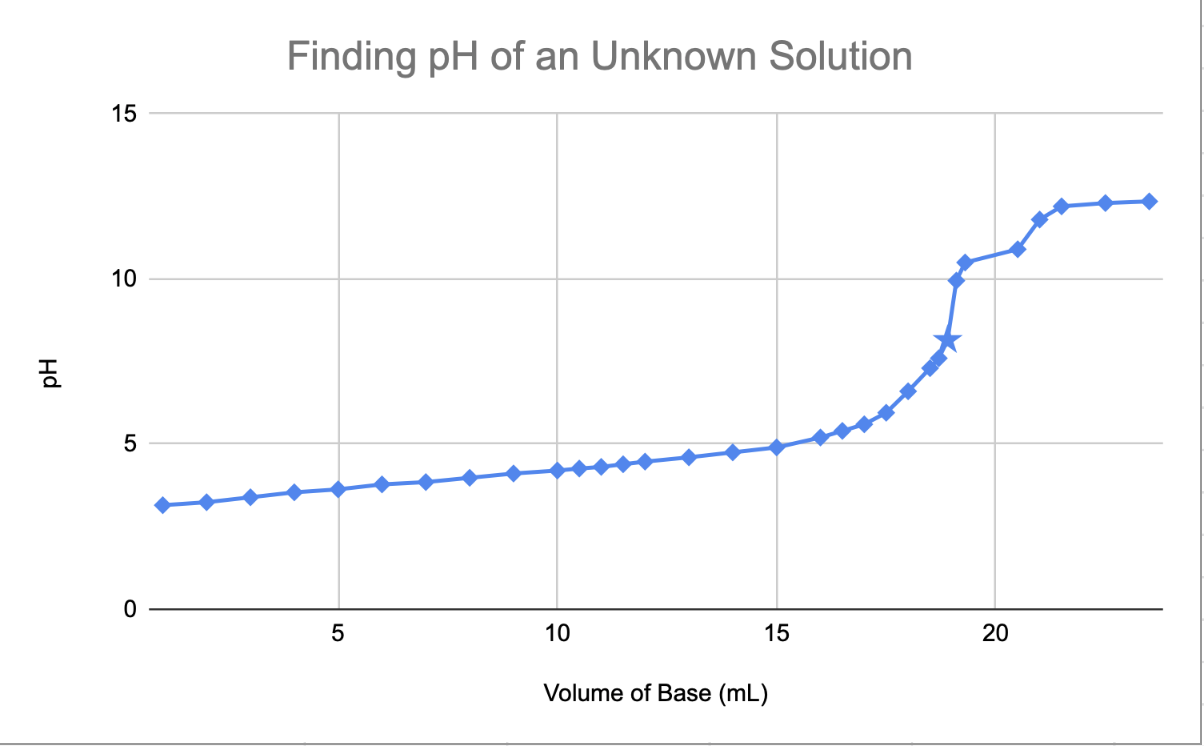
\includegraphics[width=0.48\textwidth]
{titration}
\end{figure}

\subsubsection{Mathematical Formulas}
One of the last topics to discuss is including complicated mathematical formulas into your documents. It is recommended that you include a math package if you are writing complicated mathematical formulas. One such package is \cite{Overleaf:Tutorial}:
\begin{verbatim}
\usepackage{mathtools}
\end{verbatim}
\par
Once you have your package included in your document you are ready to start writing some formulas. There are two main ways to implement formulas into your writing. First you may want your formula inline with your text like this: \(1+1=2\). Second, you may wish to have your formulas displayed on their own line like this: \[1+1=2\]
To accomplish this, we need to implement environments. The following environment is used for inline formulas \cite{Overleaf:Tutorial}:
\begin{verbatim}
\begin{math}
\end{math}
\end{verbatim}
The environment for formulas on their own line is:
\begin{verbatim}
\begin{displaymath}
\end{displaymath}
\end{verbatim}
\par
Writing all of these environments can get tiresome. Luckily, there are shorthand codes that will implement the same features without the need of incorporating math environments. Using shorthand keeps you from having to declare an environment and allows you to more easily write your formulas with the formatting you desire. The short hand for inline formulas is \cite{LaTeX2e:reference}:
\begin{verbatim}
\(...\)
\end{verbatim}
The shorthand for putting formulas on their own line is:
\begin{verbatim}
\[...\]
\end{verbatim}
\par
Most of the basic mathematical symbols are easily typed from your keyboard; however, there are many symbols not easily typed. On the next page is a table of some of the most common symbols and their commands \cite{LaTeX2e:reference}.
\begin{table}[!h]
\centering
\begin{tabular}{ |c|c| }
\hline
\$\textbackslash{}forall\$ & $\forall$\\
\hline
\$\textbackslash{}in\$ & $\in$\\
\hline
\$\textbackslash{}exists\$ & $\exists$\\
\hline
\$\textbackslash{}leq\$ & $\leq$\\
\hline
\$\textbackslash{}geq\$ & $\geq$\\
\hline
\$\textbackslash{}epsilon\$ & $\epsilon$\\
\hline
\$\textbackslash{}alpha\$ & $\alpha$\\
\hline
\$\textbackslash{}beta\$ & $\beta$\\
\hline
\$\textbackslash{}gamma\$ & $\gamma$\\
\hline
\$\textbackslash{}pi\$ & $\pi$\\
\hline
\$\textbackslash{}Pi\$ & $\Pi$\\
\hline
\$\textbackslash{}varphi\$ & $\varphi$\\
\hline
\$\textbackslash{}mu\$ & $\mu$\\
\hline
\$\textbackslash{}Phi\$ & $\Phi$\\
\hline
\$\textbackslash{}Delta\$ & $\Delta$\\
\hline
\end{tabular}
\end{table}
\par
Besides symbols there are many mathematical operators not found on your keyboard. Below is a table of some of the most common operators and their commands. \cite{LaTeX2e:reference}
\begin{table}[h]
\centering
\begin{tabular}{ |c|c| }
\hline
\$\textbackslash{}cos\$ & $\cos$\\
\hline
\$\textbackslash{}sin\$ & $\sin$\\
\hline
\$\textbackslash{}theta\$ & $\theta$\\
\hline
\$\textbackslash{}lim\textbackslash{}limits\_\{x \textbackslash{}to \textbackslash{}infty\}\$ & $\lim\limits_{x \to \infty}$\\
\hline
\$\textbackslash{}exp\$ & $\exp$\\
\hline
\$\textbackslash{}bmod\$ & $\bmod$\\
\hline
\$\textbackslash{}equiv\$ & $\equiv$\\
\hline
\end{tabular}
\end{table}
\par
When using powers and indices, you can use the \^{} symbol and \_ symbol. For example \(2^2\) is written as \cite{Overleaf:Tutorial}:
\begin{verbatim}
    2^2
\end{verbatim}
The subscript, \(k_{n-1}\), is written as:
\begin{verbatim}
    k_{n-1}
\end{verbatim}
\par
To create a fraction in LaTeX, you can write it like \textbackslash{}frac\{numerator\}\{denominator\}. For example if we wanted to write an equation like \(\frac{1}{2}*\frac{1}{2}=\frac{1}{4}\) we would write it like this:
\begin{verbatim}
    \frac{1}{2}*\frac{1}{2}=
    \frac{1}{4}
\end{verbatim}
\par
Lets put everything we have learned together and write some fairly complicated mathematical formulas. Lets try to write the following formula in LaTeX: \[\frac{n!}{k!(n-k)!} = \binom{n}{k}\]
To accomplish this we need to cover one more command. The command \textbackslash{}binom\{numerator\}\{denominator\} will allow us to end this equation properly. \cite{Overleaf:Tutorial} Here is the complete LaTeX code to write this equation using everything we have covered so far:
\begin{verbatim}
\frac{n!}{k!(n-k)!} = \binom{n}{k}
\end{verbatim}
Let try another complicated equation:
\[_{3}F_{2}\left[\begin{matrix}a& &b& &c\\&d& &e\end{matrix};z\right]\]
To write this hyper-geometric function a little creativity and the use of matrices are required. We have already covered how to write the beginning portion of this. To write \(_{3}F_{2}\), we will use the following code:
\begin{verbatim}
    _{3}F_{2}
\end{verbatim}
Next we need to tackle the matrix. To start a matrix we need to decide what type of braces we want to use. For a matrix with () braces, we would write \cite{Overleaf:Tutorial}:
\begin{verbatim}
    \left(...\right)
\end{verbatim}
This will start and stop our matrix with the symbols ( and ). Similarly we can use the [ and ] braces using the following code \cite{Overleaf:Tutorial}:
\begin{verbatim}
    \left[...\right]
\end{verbatim}
The next step is to implement the matrix. We do this by writing the environment matrix like so \cite{Overleaf:Tutorial}:
\begin{verbatim}
    \begin{matrix}...\end{matrix}
\end{verbatim}
The next step is to add the content of our matrix. This is where we need to get a little creative as LaTeX automatically wants to align all of the elements. By using the \& symbol we can adjust the alignment of each cell. For example \cite{LaTeX2e:reference}:
\begin{verbatim}
    a& &b& &c\\&d& &e
\end{verbatim}
This will separate the cells of our matrix into 2 rows and align the d and e characters under the spaces between a\&b and b\&c. Lastly we want to include the ;z in our equation. We do this by putting it outside our matrix environment but before we close the ] brace. Here is the complete code:
\begin{verbatim}
    _{3}F_{2}\left[\begin{matrix}
    a& &b& &c\\&d& &e\end{matrix}
    ;z\right]
\end{verbatim}


\subsection{References and Acknowledgements}
\subsubsection{How To - References}
\IEEEPARstart{A}{s} we near the end of this tutorial it is important that we cover how to create a proper reference section. Lets start by creating a reference environment:
\begin{verbatim}
    \begin{thebibliography}{1}
    ...
    \end{thebibliography}
\end{verbatim}
Here the \{1\} represents the number of sources used. Inside this environment, we need to add our sources that we referenced in the making of our document. \cite{Overleaf:Tutorial} We should start by setting up the first bibitem like so:
\begin{verbatim}
\bibitem{reference name}
...biliography text goes here...
\end{verbatim}
By setting up this bibitem, we are now able to cite this sort throughout our document. For example, let's say I had a bibitem named \textbackslash{}bibitem\{thehowtobook\}, I could now use the following code throughout my document to cite where I used information from this source \cite{Overleaf:Tutorial}:
\begin{verbatim}
    \cite{thehowtobook}
\end{verbatim}

\subsubsection{How To - Acknowledgements}
\par
After you have completed your references section, you may want to add an acknowledgments section. To do this, use the following code to create the new section \cite{Overleaf:Tutorial}:
\begin{verbatim}
\section*{Acknowledgements}
\end{verbatim}
The use of the * symbol here allows us to add this new section without numbering it or adding it to a Table of Contents. \cite{LaTeX2e:reference} This section is designed for you to thank whoever may have helped in the creation of your document. 

\section{Conclusion}
\IEEEPARstart{T}{he} intent of this document was to help novice engineering students with creating their first document in LaTeX. We covered what software to use and how to properly setup your document. We discussed how to begin writing content and how to properly format it for readability. We also discussed more advanced topics like the inclusion of tables, figures, and complicated mathematical formulas. LaTeX is a very powerful tool that is an industry standard for technical writing. There are many additional features that were not covered in this basic tutorial. Overleaf is a great resource for discovering more advanced techniques and features. \cite{Wikipedia:Overview}  





%\documentclass{} precedes the preamble and is typically the first command in any .tex document. Every .tex document should include this command as it defines what kind of document you intend on creating. Modifiers in square brackets [] can be added in between the text ''documentclass'' and the curly brackets {} to modify font size, templates, etc. 

% FIGURES:

% Note the FIGURE Environment created by the \begin{figure} and \end{figure} commands.

%\begin{figure}[h] 	% There are several different modifiers that can be used in [].
%\centering
%\includegraphics[width=1.5in]{slug.pdf}
%\caption{Sammy the Slug}
%\label{fig_slug}
%\end{figure}

% You will need to use appropriate file types for figures and will also need to include that image file in the same folder as your .tex file. 

%-------------------------------------------------------------------------------------------------
%\subsection{Label, Cite, and Ref Commands}
%You will need to be able to define and explain how to use the following commands:
%\begin{verbatim} \label{fig_slug} \end{verbatim} as it appears in the figure environment\\
%\begin{verbatim} \cite{IEEEhowto:kopka} \end{verbatim} appears like: %\cite{IEEEhowto:kopka}\\
%\begin{verbatim} \ref{fig_slug} \end{verbatim} appears like: \ref{fig_slug}\\

% IMPORTANT NOTE: In order to assign the correct reference number to each label, you may have to compile your code twice. 

%-------------------------------------------------------------------------------------------------
%\subsection{Tables}
%An example of a floating table.

% An example of a floating table. Note that, for IEEE style tables, the 
% \caption command should come BEFORE the table. Table text will default to
% \footnotesize as IEEE normally uses this smaller font for tables.
% The \label must come after \caption as always.
%
%\begin{table}[h]
%% increase table row spacing, adjust to taste
%\renewcommand{\arraystretch}{1.3}
% if using array.sty, it might be a good idea to tweak the value of
%\extrarowheight as needed to properly center the text within the cells
%\caption{An Example of a Table}
%\label{table_example}
%\centering
%% Some packages, such as MDW tools, offer better commands for making tables
%% than the plain LaTeX2e tabular which is used here.
%\begin{tabular}{|c||c|}
%\hline
%One & Two\\
%\hline
%Three & Four\\
%\hline
%\end{tabular}
%\end{table}


% Note that IEEE does not put floats in the very first column - or typically
% anywhere on the first page for that matter. Also, in-text middle ("here")
% positioning is not used. Most IEEE journals use top floats exclusively.
% However, Computer Society journals sometimes do use bottom floats - bear
% this in mind when choosing appropriate optional arguments for the
% figure/table environments.
% Note that, LaTeX2e, unlike IEEE journals, places footnotes above bottom
% floats. This can be corrected via the \fnbelowfloat command of the
% stfloats package.


%\section{Conclusion}
%Conclusion goes here.

%----- APPENDICES --------------------------------------------------------------------------------
%\appendices
%\section{Appendix Title}
%Appendix one text goes here.

% you can choose not to have a title for an appendix
% if you want by leaving the argument blank
%\section{}
%Appendix two text goes here.


%----- ACKNOWLEDGEMENT SECTION -------------------------------------------------------------------
% Explain what the asterisk * does in the next line: 
\section*{Acknowledgements}

I would like to thank Overleaf for providing in-depth tutorials on all things LaTeX. I would also like to thank the TeX Stack Exchange page for providing a forum to ask and answer questions regarding latex. (https://tex.stackexchange.com)

%Reminder: you will need to explain how to include an Acknowledgement Section and then include your own Acknowledgement Section at the end of your own tutorial. Same applies for the References/Bibliography.


%----- BIBLIOGRAPHY ------------------------------------------------------------------------------

% You will need to explain how to include the bibliography section as follows. Explain the environment and how to add new items.
% Including how \ref, \cite and \label should be included here.

% Reminder: you will need to explain how to include the Bibliography Section and then include your own Bibliography at the end of your own tutorial.

\begin{thebibliography}{3}

\bibitem{Overleaf:Tutorial}
Documentation. (n.d.). Retrieved January 29, 2020, from https://www.overleaf.com/learn/latex/Main\_Page
  
\bibitem{Wikipedia:Overview}
LaTeX. (2020, January 29). Retrieved January 29, 2020, from https://en.wikipedia.org/wiki/LaTeX

\bibitem{LaTeX2e:reference}
LaTeX2e unofficial reference manual (November 2018). (n.d.). Retrieved January 29, 2020, from https://latexref.xyz/

\end{thebibliography}

%----- Optional: BIOGRAPHY Section ---------------------------------------------------------------
 
% If you have an EPS/PDF photo (graphicx package needed) extra braces are
% needed around the contents of the optional argument to biography to prevent
% the LaTeX parser from getting confused when it sees the complicated
% \includegraphics command within an optional argument. (You could create
% your own custom macro containing the \includegraphics command to make things
% simpler here.)
%\begin{biography}[{\includegraphics[width=1in,height=1.25in,clip,keepaspectratio]{mshell}}]{Gerald Moulds}
% or if you just want to reserve a space for a photo:

%\begin{IEEEbiography}{Gerald Moulds}
%Biography text here.
%\end{IEEEbiography}

% if you will not have a photo at all:
%\begin{IEEEbiographynophoto}{John Doe}
%Biography text here.
%\end{IEEEbiographynophoto}

% insert where needed to balance the two columns on the last page with
% biographies
%\newpage

%\begin{IEEEbiographynophoto}{Jane Doe}
%Biography text here.
%\end{IEEEbiographynophoto}

% You can push biographies down or up by placing
% a \vfill before or after them. The appropriate
% use of \vfill depends on what kind of text is
% on the last page and whether or not the columns
% are being equalized.

%\vfill

% Can be used to pull up biographies so that the bottom of the last one
% is flush with the other column.
%\enlargethispage{-5in}

\end{document}
